% v2-acmlarge-sample.tex, dated March 6 2012
% This is a sample file for ACM large trim journals
%
% Compilation using 'acmlarge.cls' - version 1.3, Aptara Inc.
% (c) 2011 Association for Computing Machinery (ACM)
%
% Questions/Suggestions/Feedback should be addressed to => "acmtexsupport@aptaracorp.com".
% Users can also go through the FAQs available on the journal's submission webpage.
%
% Steps to compile: latex, bibtex, latex latex
%
\documentclass[prodmode,acmtap]{acmlarge}

\usepackage[utf8x]{inputenc}
\usepackage[italian]{babel}

% Metadata Information
\acmVolume{1}
\acmNumber{1}
\acmArticle{1}
\articleSeq{1}
\acmYear{2013}
\acmMonth{6}

% Package to generate and customize Algorithm as per ACM style
\usepackage[ruled]{algorithm2e}
\SetAlFnt{\algofont}
\SetAlCapFnt{\algofont}
\SetAlCapNameFnt{\algofont}
\SetAlCapHSkip{0pt}
\IncMargin{-\parindent}
\renewcommand{\algorithmcfname}{ALGORITHM}


% Title portion
\title{Relazione sul Progetto di Sistemi di Simulazione:\\Analisi della stabilità del protocollo di DHT Symphony}
\author{MATTEO BRUCATO e MIRO MANNINO\affil{Università di Bologna}
}


\begin{abstract}
Symphony è un protocollo di overlay per sistemi peer-to-peer in grado di mantenere una tabella hash distribuita (DHT) attraverso nodi che risiedono in una rete geografica.
\end{abstract}

%\category{H.5.2}{Information Interfaces and Presentation}{User
%Interfaces}[Evaluation/\break methodology]
%\category{H.1.2}{Models and Principles}{User/Machine Systems}[Human Information Processing]
\category{}{}{}[]

%\terms{Human Factors}
%\keywords{Contour perception, flow visualization, perceptual theory, visual cortex, visualization}

%\acmformat{Daniel Pineo, Colin Ware, and Sean Fogarty. 2010. Neural Modeling of Flow Rendering Effectiveness.}

\begin{document}

%\begin{bottomstuff}
%This work is supported by the Widget Corporation Grant \#312-001.\\
%Author's address: D. Pineo, Kingsbury Hall, 33 Academic Way, Durham,
%N.H. 03824; email: dspineo@comcast.net; Colin Ware, Jere A. Chase
%Ocean Engineering Lab, 24 Colovos Road, Durham, NH 03824; email: cware@ccom.unh.edu;
%Sean Fogarty, (Current address) NASA Ames Research Center, Moffett Field, California 94035.
%\end{bottomstuff}


\maketitle


\section{Introduzione}
% Cos'è Sympony e cosa vogliamo verificare con la simulazione (stabilità, perché?)

Symphony~\cite{symphony} è un protocollo per tabelle hash distribuite (DHT) che, attraverso una rete di overlay costruita in base a particolari distribuzioni armoniche, è in grado di garantire lookup efficienti, poli-logaritmici nel numero di hop (salti), ovvero nella sua \emph{latenza}\footnote{In sintonia con la terminologia tipica della letteratura peer-to-peer, indichiamo col termine \emph{latenza} il numero medio di hop per l'operazione di lookup.}.

Attraverso un concetto denominato \emph{greedy routing}, è stato mostrato come sia possibile indirizzare e consegnare un messaggio ad un qualsiasi nodo in una rete in al più $O(log^2 n)$ salti (un fenomeno chiamato anche \emph{Small World})~\cite{small-world}. Symphony si basa esattamente su questi concetti, i quali vengono applicati magistralmente al caso di reti peer-to-peer e al problema di creare DHT. In particolare, Symphony è in grado di garantire una latenza di $O(\frac{1}{k} log^2 n)$ salti, dove $k=O(1)$ è il numero di link che ogni nodo mantiene verso altri nodi della rete.

Nell'articolo in cui Symphony è stato presentato~\cite{symphony}, vengono evidenziati i molteplici vantaggi del protocollo rispetto ai suoi predecessori (Chord, Viceroy, ecc.). Il vantaggio più evidente è quello di richiedere un numero costante $k=O(1)$ di link verso altri nodi della rete, a differenza di protocolli come Chord~\cite{chord} che richiedono un numero logaritmico di link uscenti.

Symphony, inoltre, è dimostrato essere \emph{scalabile} nella dimensione della rete, ..................

Infine, gli autori dichiarano anche il sistema \emph{stabile}, ovvero capace di funzionare nel caso in cui gli host si uniscano alla rete ed escano dalla rete in maniera del tutto arbitraria, tipicamente con brevi periodi di vita. Ciononostante, un'approfondita analisi dell'articolo mostra come gli esperimenti effettuati per stabilire la stabilità di Symphony offrano solamente una panoramica limitata sui possibili scenari che possano veramente essere fonte di instabilità. I test effettuati non sono tali da stressare il sistema fino ai punti più critici, in cui un'evidente instabilità possa essere misurata.

Lo scopo del presente elaborato è quello di studiare a fondo la stabilità del protocollo Symphony, e di stabilire in maniera più accurata se tale protocollo può essere veramente considerato stabile e in che misura. Più precisamente, ci poniamo l'obiettivo di valutare la stabilità del protocollo sotto carichi di stress causati da \emph{churn}, ovvero da alte frequenze di entrata e uscita dei nodi della rete. Studieremo sotto quali condizioni di stress la stabilità del protocollo vale e in quali condizioni essa comincia a vacillare.

Attraverso una serie di esperimenti in simulazione, mostreremo come il protocollo Symphony risponda molto bene a situazioni di stress causato da \emph{churn} simili a quelle testate dagli autori dei protocollo. E' solo con l'ausilio di un \emph{motore di churn} molto sofisticato che siamo in grado invece di stressare il sistema fino a fargli perdere la sua stabilità. I nostri esperimenti, infatti, mostrano che ..................

La relazione è organizzata nel seguente modo. In Sezione~\ref{symphony} descriveremo brevemente il protocollo Symphpny. In Sezione~\ref{stabilita} descriveremo formalmente il concetto di stabilità che sarà oggetto di valutazione del protocollo in esame. In Sezione~\ref{simulatore}, presenteremo i dettagli sul simulatore realizzato, il livello di astrazione del simulatore stesso e dettagli sulla sua realizzazione. La Sezione~\ref{risultati} raccoglierà i risultati sperimentali delle simulazioni, mentre la Sezione~\ref{conclusioni} illustrerà le nostre conclusioni.





\section{Il protocollo Symphony} \label{symphony}
% Breve introduzione ai termini del paper: join, leave, re-linking, ... tutto quello usato nel resto...
Symphony è un protocollo DHT basato su un'overlay strutturato con topologia ad anello. Gli identificatori dei nodi sono selezionati in maniera randomica uniforme nell'intervallo $[0,1)$. Ogni nodo $p_i$ con identificatore $x$ gestisce il sotto-intervallo dell'anello $(y,x]$ se $y$ è l'identificatore del peer $p_{i-1}$ immediatamente precedente al peer $p_i$. In questo modo ogni valore $x \in [0,1)$ è gestito (univocamente) da uno ed un solo peer, che chiameremo il \emph{manager} di $x$ nel resto della presente relazione.

\subsection{Collegamenti tra nodi}
I nodi della rete Symphony sono collegati tra loro secondo due tipi di link: \emph{short link} e \emph{long link}, ovvero collegamenti a breve e lungo raggio. I collegamenti short servono a creare la struttura ad anello vera e propria: un peer $p_i$ è collegato per mezzo di due short link ai due peer $p_{i-1}$ e $p_{i+1}$ (supponendo sempre aritmetica modulo $n$), ovvero il suo predecessore e il suo successore nell'anello. I collegamenti long, invece, servono a permettere salti a lunga distanza nell'anello, i quali determinano la complessità logaritmica del protocollo di routing di Symphony. I long link sono quindi la caratteristica più importante del protocollo in esame.

Ogni nodo mantiene $k \ge 1$ long link. La scelta dei peer a cui collegarsi è la peculiarità principale del protocollo Symphony. Ogni nodo, quando deve decidere a chi collegarsi per mezzo di un long link, utilizza un numero randomico $x \in [0,1)$ selezionato sulla base di una distribuzione di probabilità appartenente ad una famiglia di distribuzione armoniche, una versione continua della distribuzione discreta di Kleinberg.


\subsection{Join}
Quando un peer vuole entrare nella rete





\section{Analisi della Stabilità} \label{stabilita}
% definizione formale e pochi esempi

Nell'articolo originale~\cite{symphony}, gli autori Manku et al. testano la stabilità del protocollo Symphony in una cosiddetta \emph{rete dinamica}, ovvero una rete in cui i nodi entrano ed escono arbitrariamente. In particolare, gli autori studiano una rete di centomila nodi, ognuno dei quali ha un numero logaritmico di vicini e alterna uno stato di attività ad uno stato di inattività. I tempi di attività e inattività sono tratti da due distribuzioni esponenziali diverse, tali che i nodi restino attivi per poco tempo (in media mezz'ora) e inattivi per il resto della giornata (23 ore e mezza in media). Le distribuzioni esponenziali fanno sì che la stragrande maggioranza dei nodi rispecchino questo comportamento.

Questo setup rispecchia certamente alcuni scenari veritieri di utilizzo dei sistemi DHT. I nodi entrano nella rete una volta al giorno e vi rimangono per pochissimo tempo (forse il tempo necessario per fare una semplice ricerca e scaricare uno o due file). Ciononostante non è certamente atto a coprire la maggioranza dei casi di utilizzo possibili, specialmente quelli in cui la rete venga stressata in maniera molto più pesante. Si pensi ad esempio ad un utilizzo di una DHT da parte di altri sistemi, in sistemi distribuiti integrati fra loro. In tali situazioni, non si può fare nessuna supposizione né sugli orari di utilizzo, né sulla durata d'utilizzo o sulla frequenza di entrata nella rete.

Non solo lo scenario usato nei test dagli autori di Symhony prevede una frequenza di entrata e uscita piuttosto basse, ma gli autori assumono anche una crescita della rete molto controllata. Nei loro test, infatti, essi fanno crescere la rete in maniera lineare durante l'arco di una giornata. Alla fine della prima giornata, tutti i centomila nodi sono entrati nella rete, e vi rimangono durante tutto l'arco della giornata successiva. Durante il terzo giorno, invece, i peer vengono fatti uscire dalla rete a intervalli regolari. Non siamo riusciti ad immaginare, in questo caso, un esempio di utilizzo reale che rispecchi questo particolare test. Ma soprattutto, ancora, questo test non è atto a stressare la rete con un'adeguata frequenza di churn, o in casi di altissima e imprevedibile attività.

Infine, i test riguardanti la stabilità presenti nell'articolo considerano solo reti senza re-linking. Reputiamo molto interessante stabilire cosa accade in una rete sotto churn nel caso in cui il re-linking sia attivo, in quanto esso forza molti peer a distruggere e ricreare tutti i propri long link, i quali sono quelli che contribuiscono maggiormente alle performance del protocollo stesso.


\subsection{Modello di stabilità}

Il modello di stabilità che vogliamo considerare nel presente elaborato è più complesso e a grana più fine di quello utilizzato nel paper originale. Innanzitutto, osserviamo come il tempo di permanenza di un certo peer nella rete è ininfluente rispetto la misura di stabilità della rete. Sapere che un peer sta nella rete per mezz'ora o per un giorno non fa alcuna differenza. Ciò che può maggiormente influire sulla stabilità è il fatto che una grande quantità di peer chiedano un lookup mentre la rete è in fase di creazione a seguito di \emph{join} (entrate) e \emph{leave} (uscite) dei peer.

L'ipotesi alla base dei nostri test è che durante i join (e/o i leave) l'anello di Symphony possa avere potenziali punti di inefficienza dati dal fatto che i peer che stanno entrando non hanno ancora terminato la fase di linking necessaria alla rete per funzionare nei tempi logaritmici. Aumentare il numero di peer che fanno join o leave per istante di tempo dovrebbe quindi evidenziare tale inefficienza nelle misurazioni delle latenze dei lookup.

Ciò che quindi sembra poter avere un impatto più preponderante sulla stabilità non è il tempo di permanenza del singolo peer, ma la \emph{frequenza del fenomeno di churn} (sia esso di leave o di join). Il nostro modello, quindi, prevede di potere valutare la stabilità del sistema al variare della frequenza di join e/o di leave nel sistema.

Questo approccio offre anche numerosi vantaggi in termini di flessibilità nei test. .... [poter concentrarci sulla frequenza di churn ignorando dettagli come tempo di permanenza, orario di entrata e uscita, effettiva grandezza della rete ad ogni istante di tempo permettono di effettuare test di stabilità più generali]


\subsection{Misurare la stabilità}

Una buona rete peer-to-peer senza struttura garantisce in generale che un lookup non richieda un numero di salti maggiore del numero di nodi della rete. Nel caso pessimo, infatti, la rete invia il messaggio di lookup a tutti i peer della rete finché il peer destinatario non viene contattato. L'upper bound del lookup è cioè $O(n)$ per qualunque rete peer-to-peer non banale.

Una rete strutturata come Symphony, in generale, garantisce molto meglio: un upper bound logaritmico nel numero di salti necessari ad un singolo lookup.
Ciononostante, se $n$ peer dovessero entrare tutti contemporaneamente, prima che la rete sia riuscita a creare la struttura necessaria a garantire l'upper bound teorico, le prestazioni potrebbero essere molto peggiori del previsto, fino al caso pessimo di lookup in $O(n)$ salti, come nel caso di rete senza struttura.

Bisogna inoltre considerare che l'upper bound teorico non corrisponde per forza al numero di hop necessari, e può essere anche molto più alto (pessimistico) rispetto a ciò che avviene nella realtà. Una buona struttura e un buon protocollo possono, in media, garantire numero di salti molto minori dell'upper bound teorico.

Ciononostante, è plausibile aspettarsi che uno stress maggiore o minore del sistema possa modificare, in media, il numero effettivo di salti necessari al processamento dei lookup. Ciò potrebbe portare le prestazioni del sistema ad essere nella media più vicine all'upper bound teorico. Nel seguito ci riferiamo a questo trend, se presente e misurabile, come una forma di \emph{instabilità} di un protocollo di lookup. Di contro, un sistema è più stabile tanto più le sue prestazioni rimangono eguali indipendentemente dallo stress momentaneo subito dal sistema, e tanto più il numero di salti dell'algoritmo di lookup misurati sperimentalmente si discosti dall'upper bound teorico. Tale stress è caratterizzato, come detto in precedenza, dalla frequenza di join o di leave dei peer della rete.

Introduciamo quindi, ai fini della nostra analisi, le seguenti definizioni di \emph{stabilità}: (1) la stabilità di un singolo lookup, (2) la stabilità di una serie di misurazioni di lookup, e infine la (3) stabilità di un protocollo di DHT.

\begin{definition}{(\textsc{Stabilità di un lookup})}
Dato un certo protocollo DHT e una misurazione relativa ad un singolo lookup $(h,n)$ dove $h$ è il numero di hop (salti) del lookup e $n$ è il numero di peer presenti nella rete all'istante della terminazione del lookup, la stabilità del lookup è definita come:
$$ s(h,n) = 1 - \frac{h}{n} $$
\end{definition}

L'instabilità di un singolo lookup è data da $\frac{h}{n}$ se $h$ è il numero di hop del lookup e $n$ il numero di nodi al momento presenti nella rete. Infatti, più $h$ si avvicina ad $n$, più tale numero si avvicina ad $1$, più significa che il numero effettivo di hop si avvicina all'upper bound teorico e quindi alla nostra idea intuitiva di instabilità. La stabilità, così come appena definita, quindi è data dall'opposto della instabilità, ovvero $1 - \frac{h}{n}$.

La stabilità di una singola misurazione è zero nel caso in cui $h=n$, ovvero nel caso di massima instabilità, data da una rete in cui il protocollo DHT ha perso la sua capacità di garantire un lookup logaritmico in quanto l'effetto del churn ne ha distrutto le proprietà fondamentali. La stabilità non può mai essere minore di zero, in quanto $O(n)$ è l'upper bound dei singoli lookup, come descritto in precedenza, ovvero $h \leq n$. Essa è uguale ad $1$ nel caso in cui il numero di hop effettivi sia zero (ad esempio, il file ricercato si trova nel nodo stesso che lo sta cercando). Non può essere maggiore di $1$ poiché sia $h$ che $n$ sono sempre numeri positivi. Pertanto, vale il seguente lemma:

\begin{lemma}{\textsc{Caratterizzazione della stabilità}}
$$ 0 \leq s(h,n) \leq 1 $$
\end{lemma}

Dato un insieme di misurazioni su diversi lookup, definiamo la stabilità delle misurazioni come la media delle stabilità misurate:

\begin{definition}{(\textsc{Stabilità di un insieme di misurazioni})}
Dato un certo protocollo DHT e un insieme di $r$ misurazioni della funzionalità di lookup ${H=\{ h_1, h_2, \dots, h_r \}}$, dove $h_i$ e il numero di hop (salti) relative all'$i$-esimo lookup, e dato un insieme di $r$ misurazioni ${N=\{ n_1, n_2, \dots, n_r \}}$, tale che $n_i$ corrisponde al numero di peer presenti nella rete alla fine dell'$i$-esimo lookup, la \emph{stabilità} del protocollo è definita come:
$$ stability(H,N) = \frac{\sum_{i} s(h_i,n_i)}{r}  = 1 - \frac{\sum_{i}^{}h_i/n_i}{r} $$
\end{definition}

Diciamo che un protocollo è stabile se la sua stabilità, così come appena definita, non varia di molto al variare delle condizioni di stress della rete causate dal fenomeni di churn più o meno frequenti. Il altre parole, utilizziamo la seguente definizione:

\begin{definition}{(\textsc{Stabilità del protocollo})}
Sia dato un certo protocollo DHT e un insieme di $R$ insiemi di misurazioni $M=\{ (H_1,N_1), (H_2,N_2), \dots, (H_R,N_R) \}$ tale che ogni insieme di misurazioni $(H_i,N_i)$ sia stato effettuato ad un certo livello di stress della rete dato da una certa frequenza $f_i$ di churn. Sia $S(M) = \{ stability(H_1,N_1), stability(H_2,N_2), \dots, stability(H_R,N_R) \}$. Il protocollo è detto essere \emph{stabile} sse
$$ 2 \cdot \mathrm{Std}[S(M)] \leq \epsilon $$
per un certo $0 \le \epsilon \le 1$.
\end{definition}

Si noti che, visto che la stabilità è un valore compreso tra $0$ e $1$, $\mathrm{Std}[S(M)]$ può essere al massimo $1/2$, il che giustifica il fattore moltiplicativo $2$ presente nella definizione. Intuitivamente, la presente definizione di stabilità è parametrica rispetto ad un requisito di stabilità $\epsilon$. Se $\epsilon=1$, qualsiasi protocollo è stabile, se $\epsilon=0$ un protocollo è stabile solo se la stabilità è totalmente indipendente dalla frequenza dei churn, ovvero se il numero di hop rispetto alla grandezza della rete è sempre lo stesso indifferentemente da quanti nodi entrano o escono dalla rete per unità di tempo.

Il requisito di stabilità $\epsilon$ può essere settato liberamente a seconda dei requisiti di stabilità del protocollo, e dipende quindi maggiormente dal campo applicativo specifico della DHT. Se un protocollo è stabile per un certo $\epsilon'$, allora è stabile per ogni $\epsilon'' \le \epsilon'$. Un problema interessante in questo contesto è quindi stabilire $\epsilon^*$, ovvero il minimo valore di $\epsilon$ per cui il protocollo è stabile. Nel paragonare la stabilità di due protocolli DHT, quindi, si possono utilizzare proprio i loro rispettivi valori di $\epsilon^*$. Il protocollo con $\epsilon^*$ minore è più stabile in quanto la sua stabilità è meno dipendente dalla frequenza dei churn.












\section{Il simulatore e il livello di astrazione} \label{simulatore}

\subsection{Strumenti utilizzati}

Lo studio di simulazione è stato realizzato mediante l'uso di Omnet++ 4.2.2\cite{omnet++}. Quest'ultimo è una libreria (ed anche un framework) per C++ per creare delle simulazioni. La sua struttura modulare ha favorito la realizzazione della simulazione in esame, suddividendo le varie componenti in modo da poterle gestire limitandone la complessità. Le simulazioni sono state compilate ed eseguite in due diverse architetture: Linux e Mac OS X. Ciò ha anche favorito la stesura di un codice più robusto, in grado di gestire le diversità dei due sistemi operativi, che malgrado simili tra loro, riportano leggere differenze che evidenziano errori differenti.

Rispettando le convenzioni di Omnet++, il protocollo simulato è stato realizzato mediante l'uso di:

\begin{itemize}
	\item ~ File 'NED' per modellare le varie componenti, come la rete, i peer, i canali di comunicazione ed il churner.
	\item ~ File 'msg' che definiscono i vari messaggi che i vari peer possono mandarsi.
	\item ~ File sorgenti, contenenti le classi che implementano i vari moduli descritti nei file NED.
	\item ~ File 'omnet.ini', che permette di configurare ogni run in modo parametrico.
\end{itemize}

Le analisi dei dati di ogni simulazione sono state poi effettuate sia con gli stessi strumenti messi a disposizione da Omnet++, che da piccoli script appositamente progettati per filtrare e modificare i dati grezzi, in modo da poterli poi rappresentare graficamente mediante l'uso di gnuplot.

Inoltre, le librerie grafiche messe a disposizione hanno permesso di rappresentare in maniera graficamente efficace la rete di overlay, evidenziando i vari peer con i loro collegamenti, ed i vari messaggi scambiati. Ciò ha anche aiutato la fase di debug.

\begin{figure}
\begin{center}
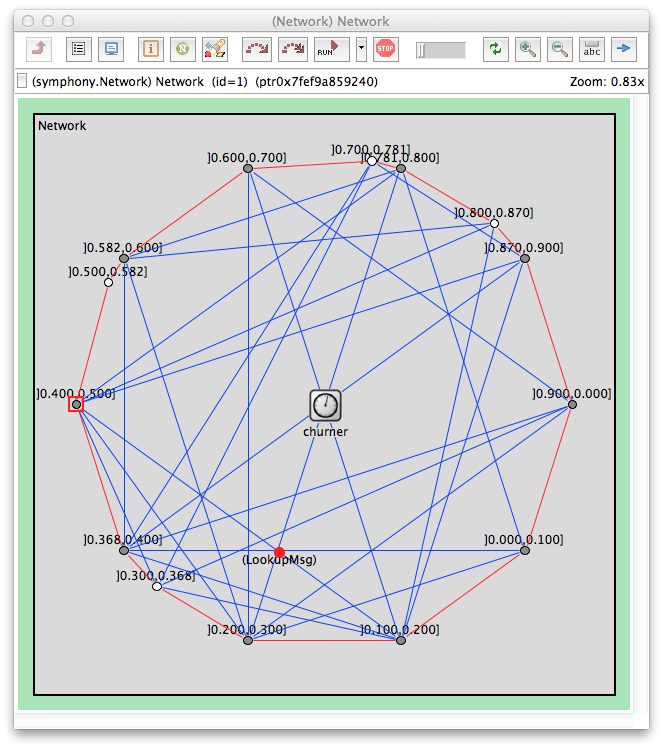
\includegraphics[scale=0.42]{imgs/screenshot.png}
\caption{Una screenshot della simulazione. Possiamo notare i long link colorati di blu ed i short link colorati di rosso. I nodi più scuri sono i peer statici, mentre quelli più chiari sono quelli dinamici. Ogni peer ha poi una label che indica il range di valori che vengono amministrati da tale nodo.}
\end{center}
\end{figure}

\subsection{Simulazione}

La simulazione è costituita da una rete, contenente una serie di peer collegati tra loro attraverso dei canali di comunicazione. Inoltre la simulazione ha un entità con un comportamento diverso dal generico peer, chiamata churner, che stabilisce quando i vari peer devono entrare ed uscire dalla rete.

La rete funge da contenitore per tutta la simulazione. Questa stabilisce il numero di peer che devono essere presenti all'interno della simulazione. Inoltre, definisce i canali presenti nella rete, con un delay di 100ms e con un bandwith di 10Mbps.

Il peer rappresenta invece un generico nodo della rete. Questa mantiene alcune informazioni necessarie per distinguersi:

\begin{itemize}
	\item ~ Un $id \in [0,1[$, che identifica univocamente il peer all'interno della rete di overlay Symphony. 
	\item ~ Un canale di comunicazione verso il nodo precedente, ed un altro per il successivo. Questi costituiscono ciò che in Symphony vengono chiamati \textit{short link}.
	\item ~ Un array di canali di comunicazione, che comunicano con peer arbitrari. Questi costituiscono ciò che in Symphony vengono chiamati \textit{long link}.
\end{itemize}

Inoltre ogni peer può contare su una serie di parametri che sono identici per ogni peer, che delineano in modo parametrico il loro comportamento finale.

\begin{itemize}
	\item ~ Il parametro \textit{k}, che costituisce il numero di long link che il peer deve provare a fare.
	\item ~ Un parametro per stabilire il numero di tentativi che il peer è disposto a fare per costruire i long link. Ciò viene accuratamente descritto nell'articolo originale di Symphony.
	\item ~ Uso o meno del relinking.
\end{itemize}

Ogni peer poi può essere utilizzato, all'interno della simulazione, in due modi piuttosto differenti: in maniera statica ed in maniera dinamica. 

\paragraph{Peer statico}
Il peer statico viene inserito all'interno della rete di overlay in maniera automatica, prima che la simulazione abbia inizio, attraverso i costrutti dei file NED. Tali nodi, inoltre, non escono mai dalla rete. I long link, invece, a causa del potere espressivo troppo debole di tali costrutti, non possono essere creati in modo corretto utilizzando il linguaggio NED (e.g. verrebbero collegati due nodi già connessi, oppure verrebbero creati più di $2k$ link entranti). Pertanto i peer statici creano questi long link all'inizio della simulazione, senza l'utilizzo di messaggi. Ciò determina una fase transiente in cui la rete statica si configura, che deve essere ignorata al fine di garantire delle misurazioni coerenti. Per questo motivo, le simulazioni attendono un \textit{periodo di warmup}. In particolare anche il churner deve attendere tale periodo prima di far entrare ed uscire i peer dinamici.

Ogni peer statico $p_i$ ha inizialmente un $id_i \in [0,1[$ ben preciso: se rappresentiamo i peer statici come $\{sp_1, \linebreak[1] sp_2, \linebreak[1] ..., \linebreak[1] sp_n\}$, abbiamo che $id_i = i / n$. Ciò significa che gli id dei peer statici sono uniformemente distribuiti all'interno dell'anello che rappresenta la rete di overlay di Symphony.

\paragraph{Peer dinamico}
I peer dinamici vengono inseriti all'interno della rete che contiene tutti i peer della simulazione, ma non all'interno della rete di overlay. Pertanto inizialmente ognuno di essi non ha long link o short link. 

Un generico peer dinamico rimane quindi in disparte fino a quando il churner, attraverso un messaggio, non gli chiede di entrare a far parte della rete. A quel punto, come stabilito da Symphony, questo deve assegnarsi un id e deve contattare il peer che lo amministra attualmente, attraverso un lookup, che deve partire da un peer noto  a priori. Ogni nodo dinamico utilizza come peer noto un nodo casuale tra quelli statici. Tale scelta garantisce un uniformità nel carico in questa prima fase, poiché i punti di ingresso dei lookup sono uniformemente distribuiti all'interno dell'anello, grazie anche all'inizializzazione degli id dei peer statici.

Un generico peer dinamico, dopo essere entrato all'interno della rete di overlay, rimane al suo interno fintantoché il churner non gli chiede di uscire. A quel punto il peer non deve far altro che eliminare tutti i collegamenti, ripristinando la topologia, ritornando nella sua fase iniziale, e attendendo nuovamente di poter rientrare. 

Quando il peer dinamico si trova fuori la rete può ricevere comunque dei messaggi di lookup (i.e. quelli che gli sono stati mandati poco prima la sua uscita dalla rete di overlay, e che quindi erano in transito al momento dell'uscita). Tali messaggi vengono scartati e rimandati al mittente, in modo da simulare fedelmente i tempi di un reale protocollo. In tal modo il mittente può gestire nuovamente il messaggio, inviandolo ad un peer più appropriato.

\paragraph{Churner}

Il churner è un entità esterna alla rete di overlay che non partecipa quindi alla computazione. Ciò che viene fatto da tale entità è semplicemente far entrare (e far uscire) un peer ogni $t$ secondi. La gestione del churn è stata affidata ad un'entità esterna, piuttosto che ai peer stessi, per avere una maggiore flessibilità, oltre che una maggiore precisione nei test. Infatti, gestire la frequenza di entrata e di uscita nei peer stessi, richiederebbe una complessa coordinazione tra i peer. 

La scelta del peer da far entrare (tra quelli che sono fuori la rete di overlay) è casuale. Lo stesso vale per la decisione sul peer da far uscire. In quest'ultimo caso però, non viene mai fatto uscire un peer che non ha ancora completato tutti i suoi long link.


\subsection{Livello di astrazione}

%simulazione della sola rete di overlay
La simulazione, come abbiamo visto, è composta da vari peer, collegati tra di loro mediante l'uso di short link e long link. Una prima osservazione sul livello di astrazione è pertanto quella che riguarda la topologia della rete. Nella realtà, ogni peer fa parte di una rete (e.g. Internet), differente dalla rete di overlay, creata in maniera logica da Symphony. Nella nostra simulazione viene rappresentata solamente quest'ultima, dove ogni link (sia short che long) ha un delay di 100ms ed un bandwith di 10Mbps, che abbiamo stimato essere una buona approssimazione di un usuale canale di comunicazione logico che collega due peer presenti sulla rete di Internet.

%come abbiamo risolto gli accessi a sezioni critiche
In una reale implementazione del protocollo i peer che entrano ed escono dalla rete hanno bisogno di meccanismi di accesso in sezione critica distribuiti, per non creare delle incoerenze che potrebbero intaccare negativamente la struttura della rete di overlay. Tali meccanismi sono a volte complessi da implementare e non sono oggetto del nostro studio. Per risolvere tutti gli accessi a sezione critica è stato pertanto utilizzato il fatto che, nella simulazione fatta da Omnet++, qualunque metodo non viene mai eseguito in concorrenza. Tutte le manipolazioni della topologia vengono pertanto fatte dal peer interessato, in un solo metodo, compiendo quindi un'azione atomica istantanea (ovvero impiega un tempo di simulazione nullo). 

%conoscenza del vicinato
Si assume che ogni peer all'interno della rete di overlay abbia una conoscenza dei peer che compongono il proprio vicinato. Ciò è un'assunzione realistica e comunemente utilizzata nei reali sistemi peer-to-peer. Per questo motivo ogni peer conosce l'id di ogni suo vicino, recuperato al momento della creazione del link che li ha connessi. Lo stesso non si può dire per gli id gestiti da un peer vicino, poiché tale informazione cambia continuamente. 

%che id gestisco? qual'è il peer vicino migliore per forwardare un messaggio?
Detto ciò è necessario chiarire due due cose molto importanti. La prima è sapere quali sono gli id gestiti dal proprio peer: tale informazione viene ottenuta senza l'invio di nessun messaggio, considerando il proprio id e quello del peer precedente. La seconda è sapere a chi dobbiamo fare il forward di un messaggio di lookup che richiede di cercare il manager dell'id $x$: analogamente, senza mandare messaggi, possiamo semplicemente controllare gli id di ogni peer vicino e fare il forward al peer con l'id che si avvicina maggiormente ad $x$ (come descritto dal Routing Protocol di Symphony). In una reale implementazione queste due considerazioni continuerebbero a valere, rendendo dunque questi aspetti fedelmente simulati.

\subsubsection{Messaggi}

Ogni peer può mandare diversi messaggi:

\begin{itemize}
	\item ~ \textit{LookupMsg}: è il messaggio di lookup. Tale messaggio può essere utilizzato per tre motivi diversi: per cercare il manager di un id quando viene fatto un join, per cercare il manager di un id per poter creare un long link, oppure per un lookup generico che simula la ricerca di un file all'interno della rete.
	\item ~ \textit{LookupResponseMsg}: è la risposta ad un lookup, che trasporta al suo interno l'identificatore del manager. In questo modo il peer che ha fatto la richiesta può compiere un azione opportuna.
	\item ~ \textit{NEstimationMsg}: è il messaggio che viene spedito per aggiornare la stima del numero di peer presenti all'interno della rete, come previsto dal protocollo di Symphony.
\end{itemize}

%id nei messaggi di lookup, coda dei messaggi di uscita
Ogni richiesta di lookup emessa da un determinato peer, viene identificata da un id crescente. Anche nel caso questo uscisse e rientrasse dalla rete, tale id è garantito essere distinto. Ogni peer mantiene poi una coda dei messaggi di lookup che sono stati inviati, associando ad ognuno di essi la procedura all'interno del peer che ha richiesto l'invio di tale messaggio. Ogni risposta di un lookup (i.e. LookupResponseMsg) mantiene al suo interno questi id, permettendo al peer di identificare e continuare a svolgere tali procedure (il messaggio viene ignorato se non si dovesse trovare nella coda una corrispondenza). Inoltre, considerando che la coda di messaggi viene svuotata al momento dell'uscita dalla rete di overlay, questo meccanismo permette anche di ignorare le risposte ai lookup inviati in una precedente reincarnazione del peer, evitando il verificarsi di errori.

%join
Per utilizzare i messaggi di lookup in modo da effettuare un join, il peer segna un campo all'interno del messaggio, in modo da distinguerlo. Così facendo il manager dell'id, invece di rispondere solamente a tale lookup, manipola la topologia della rete di overlay, in modo da far entrare il peer al suo interno. Le operazioni di join non possono infatti essere fatte dal peer stesso poiché, durante il tempo trascorso per la ricezione della risposta del lookup, il manager può non gestire più l'id che gli era stato richiesto, generando conflitti che perturberebbero la topologia della rete di overlay. Il join, compiendo un'azione atomica per manipolare la topologia, utilizza un numero di messaggi che nella realtà sarebbe più alto, per via della semplificazione negli accessi a sezione critica.

%leave
L'operazione dei leave viene fatta dal peer in maniera atomica, in modo da evitare anche qui qualunque errore di concorrenza. Come il join, il numero di messaggi inviati è minore a quello che sarebbe in un protocollo reale.

%n-estimation
La stima del numero di peer all'interno della rete di overlay rispecchia fedelmente il protocollo di Symphony. In questo caso viene utilizzato il messaggio NEstimationMsg per mandare tali stime ai peer coinvolti in un join.


\section{Risultati} \label{risultati}


\section{Conclusioni} \label{conclusioni}












% Appendix
%\appendix
%\section*{APPENDIX}
%\setcounter{section}{1}



% Bibliography
\bibliographystyle{ACM-Reference-Format-Journals}
\bibliography{bibliografia}

% History dates
%\received{February 2009}{July 2009}{October 2009}




%\elecappendix


%\section{Analysis of Invalid Trials}
%\label{invalid}

%\subsection{Results}




\end{document}
% End of v2-acmlarge-sample.tex (March 2012) - Gerry Murray, ACM
